
\section{Trapped Ion Quantum Computing} \label{sec:Trapped}
In this section we provide an introduction to the implementation details of trapped ion quantum computers (**once done possibly elaborate what exactly we cover).
The qubits in a trapped ion system are represented by individual trapped ions.
As would have been seen in a quantum mechanics class, electrons bound in atoms can occupy a certain number of possible quantum states, here 2 of these level are chosen and used as the \kz and \ko states.
Though it isn't quite as simple as that, for quantum computing we must have a way of entangling these 2 states.
To achieve that, the qubit ions are trapped in the same trap and their motion within it is coupled as a quantum system, through which entanglement is achieved.
The rest of the required features for quantum computing including state preparation, readout and quantum gates are all achieved through tuned lasers (we use the word a bit loosely, it is to mean any source of a particular type of light) and or the mentioned entanglement.
The section is largely based on the review by Brunzewicz \cite{bruzewiczTrappedionQuantumComputing2019} and for a more detailed review on the subject we recommend that.

\subsection{Ion Trapping and the Paul Trap}
\textbf{TODO: Also, a section on cooling might be a good idea}

Ion trapping is an extensive field of expertise used for many purposes across physics and other sciences, it is an essential component of many devices and experiments that try to manipulate individual particles, molecules or so on.
For a brief sketch of what this involves, these experiments must be done in vacuum (otherwise there would be too many other atoms around) and rely on complex electric and magnetic fields to manipulate the motion of charged atoms.
For quantum computing we are interested in trapping individual ions in a stable way, and while we want to trap multiple of them (currently about 5-100 has been achieved \cite{paganoCryogenicTrappedionSystem2018}) it is important that we can tell them apart (as opposed to trapping them in bunches as is often done).

There are currently 2 dominant, suitable classes of ion traps, Penning traps which uses a combination of magnetic and electric fields, and Paul traps (also known as Quadrupole or Radio-Frequency-Quadrupole ion traps) which uses time varying electric fields.
Penning traps are able to hold larger amounts of ions and more stably (300 ion crystals have been achieved \cite{bohnetQuantumSpinDynamics2016}), however the motion of the ions themselves is much more complicated and leads to qubit manipulation being harder to perform.
Because of that Paul traps are more commonly used for quantum computers and due to the scope of this report we will focus on them.

\subsubsection{Simple Paul Trap}
Paul trap designs use time varying fields as it is not possible to confine an ion in 3D space with only static fields.
The simplest Paul trap design is composed of 4 conducting rods run in parallel to create a quadrupole electric field in the middle (\cref{fig:TIQC_RFQ_Flour} shows a demonstrative model).
Then have each of the diagonally opposite rods connected at the same voltage and have these 2 voltages be some periodic function (usually a sine or a square wave at approximately radio frequencies, hence the name) in antiphase, so that if at some time one pair is set to positive voltage, the other should be at negative voltage.
This results in a net effect of trapping a charged particle (within some range of mass to charge ratios of the ions, the setup can be used as a mass filter) along the axis of the quadrupole, why exactly this is so is well explained in (**add a source here).
Finally, for trapping along the last axis a static electric field is used, this can be achieved by for example 2 more rod segments along the quadrupole axis at either end of the whole setup, both at some positive voltage, resulting in a potential well along the axis.

\begin{figure}[h]
    \centering
    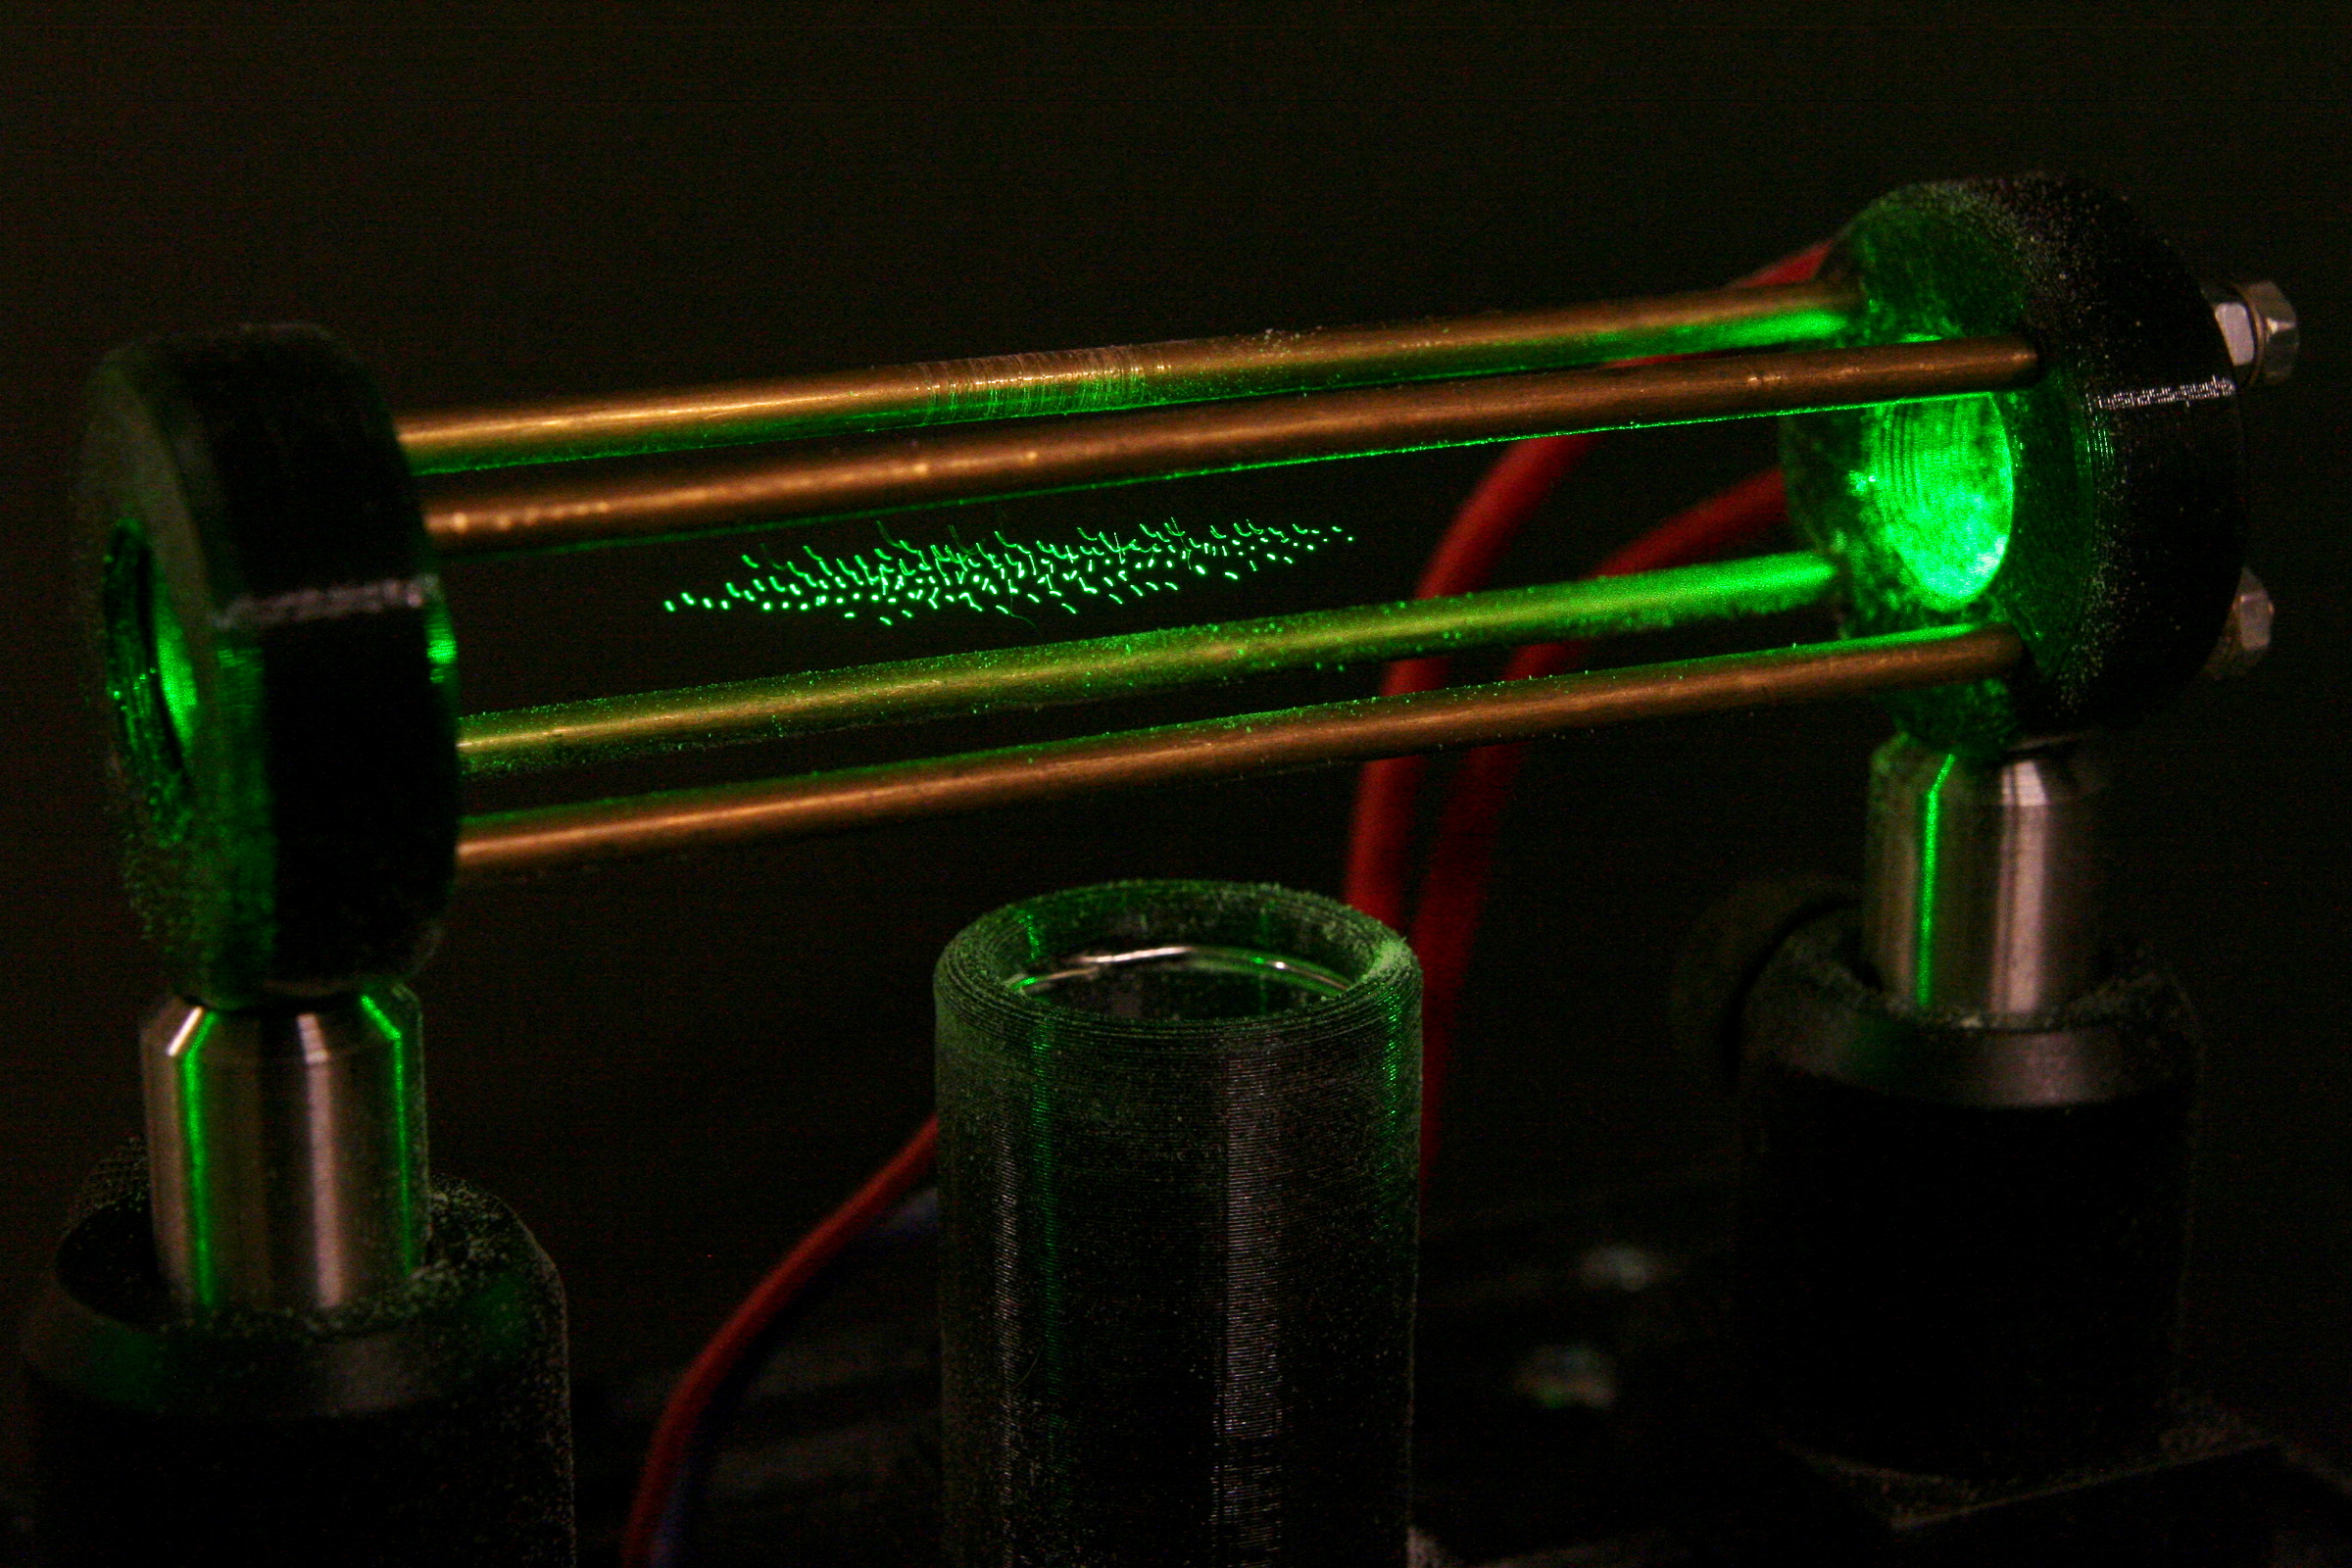
\includegraphics[width=0.9\textwidth]{images/TIQC_RFQ_Flour.jpg}
    \caption{Charged flour grains trapped in a simple Paul trap, the mentioned 4 parallel rods are visible and the electrodes creating the potential well are in the end caps.(**cite Pavelka, found on wikipedia)}\label{fig:TIQC_RFQ_Flour}
\end{figure}

\subsubsection{Notes on Other Paul Trap Designs} \label{sec:other_paultraps}
The aforementioned simple Paul trap is in fact a linear Paul trap, in this type of Paul traps the ion's motion is confined in 2 dimensions by an RF quadrupole and the last is taken care of using a linear static potential, this is the type of trap on which we will focus.
There are also point Paul traps, which utilise oscillating RF fields for trapping in all 3 dimensions, these are also used for quantum computing, however when multiple ions are trapped together (which is necessary for entanglement) their motion is significantly more complex.

However there is still a plethora of different designs being explored for further progress, most interestingly there are "surface" Paul traps.
These are usually microfabricated plates with a layout of electrodes on their surface which when driven by the correct voltages give rise to a trapping field above their surface.
These designs offer great advantages for quantum computing, as not only are they cheaper and quicker to manufacture, but can be produced with a much higher precision than manually assembled devices.
They also have the benefit of the trapped ions being much more accessible for manipulation through lasers.
Recently chips with integrated photonics have been developed too, these are surface Paul traps with optical channels running through them with openings in the surface aimed at the ion see \cref{fig:TIQC_MIT} for diagrams of one developed at MIT \cite{niffeneggerIntegratedMultiwavelengthControl2020}.
This further reduces the need for precision assembly and calibration, however complications arise with generating and maintaining entangled states if each ion is stored separately in these modules \cite{bruzewiczTrappedionQuantumComputing2019}.


\begin{figure}[h]
    \centering
    \begin{subfigure}[b]{0.45\textwidth}
        \centering
        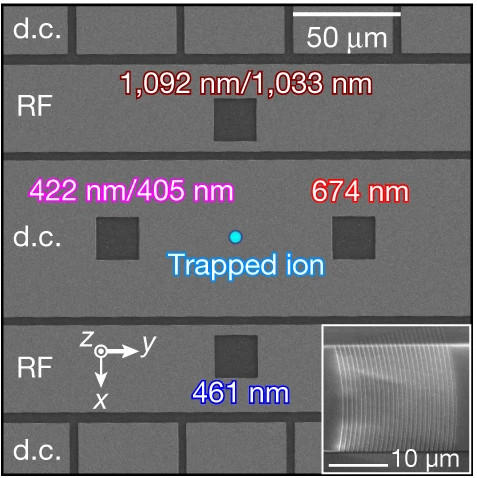
\includegraphics[width=0.9\textwidth]{images/TIQC_MIT_1.jpg}
        \subcaption{Layout of the surface Paul trap}
    \end{subfigure}
    \hfill
    \begin{subfigure}[b]{0.45\textwidth}
        \centering
        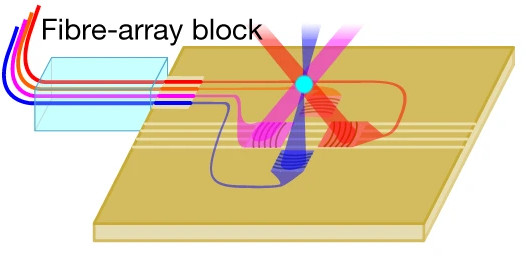
\includegraphics[width=0.9\textwidth]{images/TIQC_MIT_2.jpg}
        \subcaption{Diagram showing the photon beams}
    \end{subfigure}
    \caption{Surface Paul trap with integrated photonics for quantum computing developed at MIT in 2020.}\label{fig:TIQC_MIT}
\end{figure}

\subsection{The ions and types of qubits}
As the trapping was briefly covered, the next logical step is to focus on the ion itself.
First question is what element should be use and some of the main requirements are that it is radioactively stable, can be easily produced and singly ionized and finally that it has 2 suitable states to use as \kz and \ko from the DiVincenzo criteria.
For this, the valence electron (also the one that is "free" due to ionization) is the important part, the energy levels available to it are used as our needed states.
Typically, group 2 elements or similar (namely group 12 elements and Yb \cite{ozeriTrappedionQubitTool2011}) are used, as they are stable and have a full shell except a single valence electron -- leading to a suitable electronic structure.

For a quick summary of atomic structure, an electron is bound to the nucleus by the Coulomb interaction, if this is considered only and the quantum problem is solved, we get the gross structure, giving rise to different energy levels with different quantum numbers n.
The next step is to consider the interaction between the electrons spin and angular momentum, and also certain relativistic corrections.
This gives rise to the fine structure which are the usual orbitals described by the quantum numbers: the same n, l usually given letters s, p, d and so on, and the total spin j.
Next, there is another correction which comes from the interaction between the electron's spin and the total spin of the nucleus (if non-zero).
This gives rise to more splitting and the resulting energy levels are called the hyperfine structure.
Finally, in very vague terms, if an atom is in a magnetic field there is again more splitting, this is called the Zeeman effect.
Details on all of this can be found in \cite{woodgateELEMENTARYATOMICSTRUCTURE1970} and a diagram of the typical fine structure of the ions used for trapped ion QC along with some of the zeeman and hyperfine splittings are shown in \cref{fig:TIQC_levels}.

% some of the main requirements for a suitable isotope is that it is radioactively stable, can be produced, is singly ionizable and most importantly that the valence electron has suitable stable available quantum mechanical states to occupy, to use for \kz and \ko.
% However for many of them, there are multiple suitable electron states available for use, based on which are used the qubits would be classified as Zeeman, Hyperfine, Optical or Fine-structure.
% To summarize what these are, in either case we start with the typical electron orbitals around an atom

This gives rise to a plethora of options for the 2 levels and depending on their choice the resulting qubit can be classified into the following categories.

% Coming back to quantum computing there are many options for our states and they can usually be classified as one of following types.

\begin{figure}[h]
    \centering
    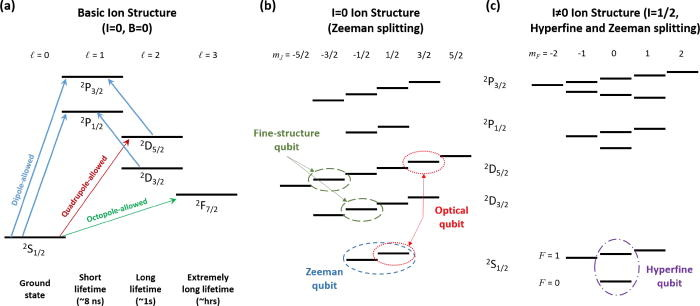
\includegraphics[width=0.9\textwidth]{images/TIQC_levels.jpeg}
    \caption{Fine structure and Zeeman and hyperfine splittings of typical atoms used for quantum computing. Some of the possible choices for the sates are also shown.}\label{fig:TIQC_levels}
\end{figure}

\paragraph{Zeeman qubits}
Zeeman qubits are qubits where the 2 states are in the same hyperfine and fine structure orbital, but result from the Zeeman effect.
They offer near infinite lifetimes and most operations can be done relatively simply, but their main drawback is that these states are very sensitive to magnetic field fluctuations (they arise from external magnetic fields after all).
This limits their coherence times, however coherence times of 300 ms have been achieved \cite{rusterLonglivedZeemanTrappedion2016}

\paragraph{Hyperfine qubits}
With these the 2 states are hyperfine split levels from the ground state.
Among their advantages are also an near infinite lifetime and possibly and an easier read out than Zeeman qubits along with a relative insensitivity to magnetic field fluctuations.
The main drawback to them is the more complicated structure of the energy levels, thus requiring greater precision in laser frequencies \cite{bruzewiczTrappedionQuantumComputing2019}.

\paragraph{Optical qubits}
In some ions it is possible to use an S and a D level as our states, this has the benefit of very simple level structure.
However these D states are only metastable, of lifetimes on the order of seconds \cite{ozeriTrappedionQubitTool2011}.
Furthermore, the more precise the laser frequencies are the longer the achieved lifetimes are, however as the energy gap is relatively large for these states, the required lasers for manipulation need to have frequencies of visible to infrared light (hence the name).
The long wavelength of the manipulating lasers also results in less localised beams ($\lambda \sim \si{m}$) which means it is tough to address individual ions (cite oxford thesis 2).
As suitable laser precisions are very hard to attain optical qubits tend to be less popular, however their popularity is growing with advances in laser sources \cite{bruzewiczTrappedionQuantumComputing2019}.
% However as the energy gap gets bigger so does the required lasers wavelength and for optical qubits the frequencies are of visible to infrared light (hence the name) and achieving the required frequency precision is a very difficult task.

\paragraph{Fine structure qubits}
This type of qubit uses 2 of the D levels mentioned in the last section.
The obvious downside is then their short lifetimes, however as the energy gap between these levels is much smaller, higher frequency precision can be more easily attained in the required lasers.
As a downside comes a more complicated level structure, for example the readout has to be done by first transferring one of the possible states to another one before reading out.


Overall there is not a clear winner and which choice is made depends on the particulars of the given company or research team, depending on their expertise and the equipment available to them.


\subsection{Qubit manipulation and ion-light interactions}
In the previous sections we have described how we achieve the necessary 2 states from the 1st DiVincenzo criteria, however we still have all the others to address.
All of these (in summary they are state initialization and readout, a set of universal gates and long decoherence times) are achieved through different light beams interacting with the.
% These are quite complex and we only describe them at a fairly surface level, for more detail we recommend \cite{schaferFastGatesMixedSpecies2020} (the main source for this section) and specifically section 3.2 as an introduction to these phenomena.

Firstly, here we are considering the ions to be trapped within the same trap.
Typically this is modeled along the lines of the linear Paul trap where we only take into account motion along the z axis.
We trap some number of ions in an approximately harmonic potential\footnotemark and they form essentially a 1D crystal through the Coulomb force interactions.
It should be noted that the ions do not interact directly with each others electronic states while in the trap.
This is because they are simply too far from each other, for example \cite{schaferFastGatesMixedSpecies2020} quotes typical sizes of the ions wavefunctions to be $\sim 8 \si{\nano m}$ and the ions separations to be $\sim 3 \si{\micro m}$.

\footnotetext{This is simpler than many of the moderns systems like the ones mentioned in \cref{sec:other_paultraps}, however the while ion manipulation and entanglement is more complicated with these it is fairly analogous.}

At this point it really becomes necessary to look at the system quantum mechanically.
As the ions are within the same trap their motion is strongly coupled and can only be described together in one quantum system.
This essentially means we must look at the ions in the trap more as a collective motional wavefunction than a collection of individual atoms.
However at the same time each atoms electronic state is still kept separate and localised.
Thus we end up with essentially a register of n 2 state qubits with a shared motional state acting as a bus between them.
This motional state is also kept as simple as possible, the ions are cooled to attain the ground state and often only the first excited motional state is used for operations.

\subsubsection{Single qubit gates}
Firstly, there is not a single unified method for achieving these gates as different methods can be more suited for a particular application and choice of qubit.
Common to all of them however is that single ion gates only deal with the electronic state of a particular ion and they manipulate it by inducing transitions using light beams.
These light ion interactions are quite complex and are studied for example in \cite{loudonQuantumTheoryLight2000}, here we only try to build some intuition for them without real analysis.

As these are a quantum interactions, the key thing is to construct a Hamiltonian.
This being a complicated interaction however we don't solve it directly, instead we expand it and only look at the first (possibly couple of the first) non-zero terms, the results are taken from \cite{schaferFastGatesMixedSpecies2020}.

\paragraph{Electric dipole transitions}
The electric dipole term is the dominant term if not zero.
The analysis of the problem leads to the following quantum mechanical propagator, which can be viewed essentially as the matrix representation of the gate's effect on the ion's state,
\begin{equation}
    U = \begin{pmatrix}
        \cos{(\frac{\Omega_R t}{2})} & i \sin{(\frac{\Omega_R t}{2})} e^{-i \phi_l} \\
        i \sin{(\frac{\Omega_R t}{2})} e^{i \phi_l} & \cos{(\frac{\Omega_R t}{2})} \\
    \end{pmatrix}
\end{equation}
where $\Omega_R$ is the Rabi frequency which depends on the choice energy levels and the electric field amplitude of the incoming light, so it can be set.
Further $t$ is just the time (the effect of the light will depend on how long it was turned on for) and $\phi_l$ the phase of the laser light at the ion, so it can be manipulated by tuning the laser source position relative to the ion.
This type of propagator then results in what is called Rabi oscillations, the state will be changing in some deterministic way periodically in time.
In summary then as $\Omega_R$ and $\phi_l$ can be almost arbitrarily chosen we can choose in what way it oscillates, and by choosing the time for which the laser is kept on we can achieve any rotation of the qubit on the Bloch sphere \cite{schaferFastGatesMixedSpecies2020}.







% The system and its interaction has to be examined using quantum mechanics, for this the starting point is always the Hamiltonian/the energy of the system.
% As has been established, each ion will be in some internal state which is a superposition of the 2 levels, this gives :w.
% In addition to that, each is in a harmonic potential, thus we get a 

% As has been established, each ion is in a superposition of 2 internal states, each has a certain energy associated with it, this gives a spin-like term in the Hamiltonian - $\frac{\hbar \omega_0}{2}$ with $\hbar \omega_0$ being the energy required for the transition between the states.
% Further, each ion is in a harmonic potential so we get the usual quantum harmonic oscillator term $$



\subsection{Qubit (ion) manipulation, the lasers for state prep, readout and so on, and entanglement!}

TODO
\begin{itemize}
    \item lamb-dicke limit might be good to mention
    \item Mention DiVincezo in above, essentially what was now described is how the \kz and \ko states are stored
    \item motional states! and entanglement through them, can get long
    \item actual manipulation - ideally structure along DiVincezo
    \item redout is apparently done by "quantum jump" technique with unit efficiency - reference 11 in cirac and zoller
\end{itemize}

